

\section{Main Application Development}

In the previous sections, the following sections have been discussed: 
\begin{itemize}
	\item Introduction to the Measurement Network Gateway project
	\item Hardware used for this project
	\item Software used for development in this project
	\item The VHDL codes and the IP generated for this project
	\item Petalinux Build using the generated IP
	\item Linux Kernel Module Development for the custom built hardware
\end{itemize}

Using the Linux Kernel Module that was developed for the custom hardware, we are able to access the peripherals available on the ZedBoard. Additionally, custom VHDL modules for reading the temperature sensor, ADC0, and ADC1 have been implemented. The kernel module provides a unified interface to access all these hardware components from userspace applications through the \texttt{/dev/meascdd} device interface.

Building upon this hardware abstraction layer, this section focuses on the development of the main userspace application that forms the core of the Measurement Network Gateway system. The main application is responsible for orchestrating all software-level operations required for sensor data acquisition, management, and distribution.

The main application architecture consists of several key components working in coordination:\\

\textbf{Data Storage and Buffering:} To decouple the acquisition process from data transmission and ensure reliable operation under varying client request rates, a thread-safe ring buffer data structure has been implemented. This buffer serves as the central data repository, allowing the sensor thread to continuously produce samples while the server thread consumes them at different rates without data loss or synchronization issues.

\textbf{Sensor Acquisition and Management:} A dedicated sensor thread continuously polls the hardware peripherals through the kernel module interface at configurable sampling rates. This thread handles all low-level sensor communication, including temperature readings, ADC conversions, switch states, and push-button events. Each acquired sample is timestamped with microsecond precision and tagged with a unique sensor identifier for proper data organization.



\textbf{Network Server and Client Communication:} A TCP server thread provides network connectivity to external clients, enabling remote access to real-time sensor data and gateway configuration. The server implements a command-based protocol that allows clients to request data, configure sampling rates, and control gateway behavior. This component bridges the gap between the embedded acquisition system and remote monitoring applications.

\textbf{Configuration and Control:} The application includes a configuration management system that maintains sampling rate parameters for each sensor type. Configuration updates can be initiated both locally through a command-line interface and remotely through network commands, providing flexible control over the gateway's operation.

\textbf{Thread Synchronization and Resource Management:} Given the multi-threaded architecture with shared resources (ring buffer, configuration structures), careful synchronization using pthread mutexes ensures thread-safe access and prevents race conditions. The application implements proper lifecycle management for thread creation, execution, and termination.

In the previous sections, each of these components have been examined in detail and in this section particular emphasis will be on the network server implementation, which forms the backbone of the gateway's remote access capabilities. We begin with a comprehensive discussion of the TCP server architecture, connection management, command protocol design, and the mechanisms that enable reliable real-time data streaming to GUI clients.


\section{Architecture of the Main Application}
The following figure shows the overall software architecture of the Measurement Network Gateway. 

\begin{figure}[H]
	\centering 
	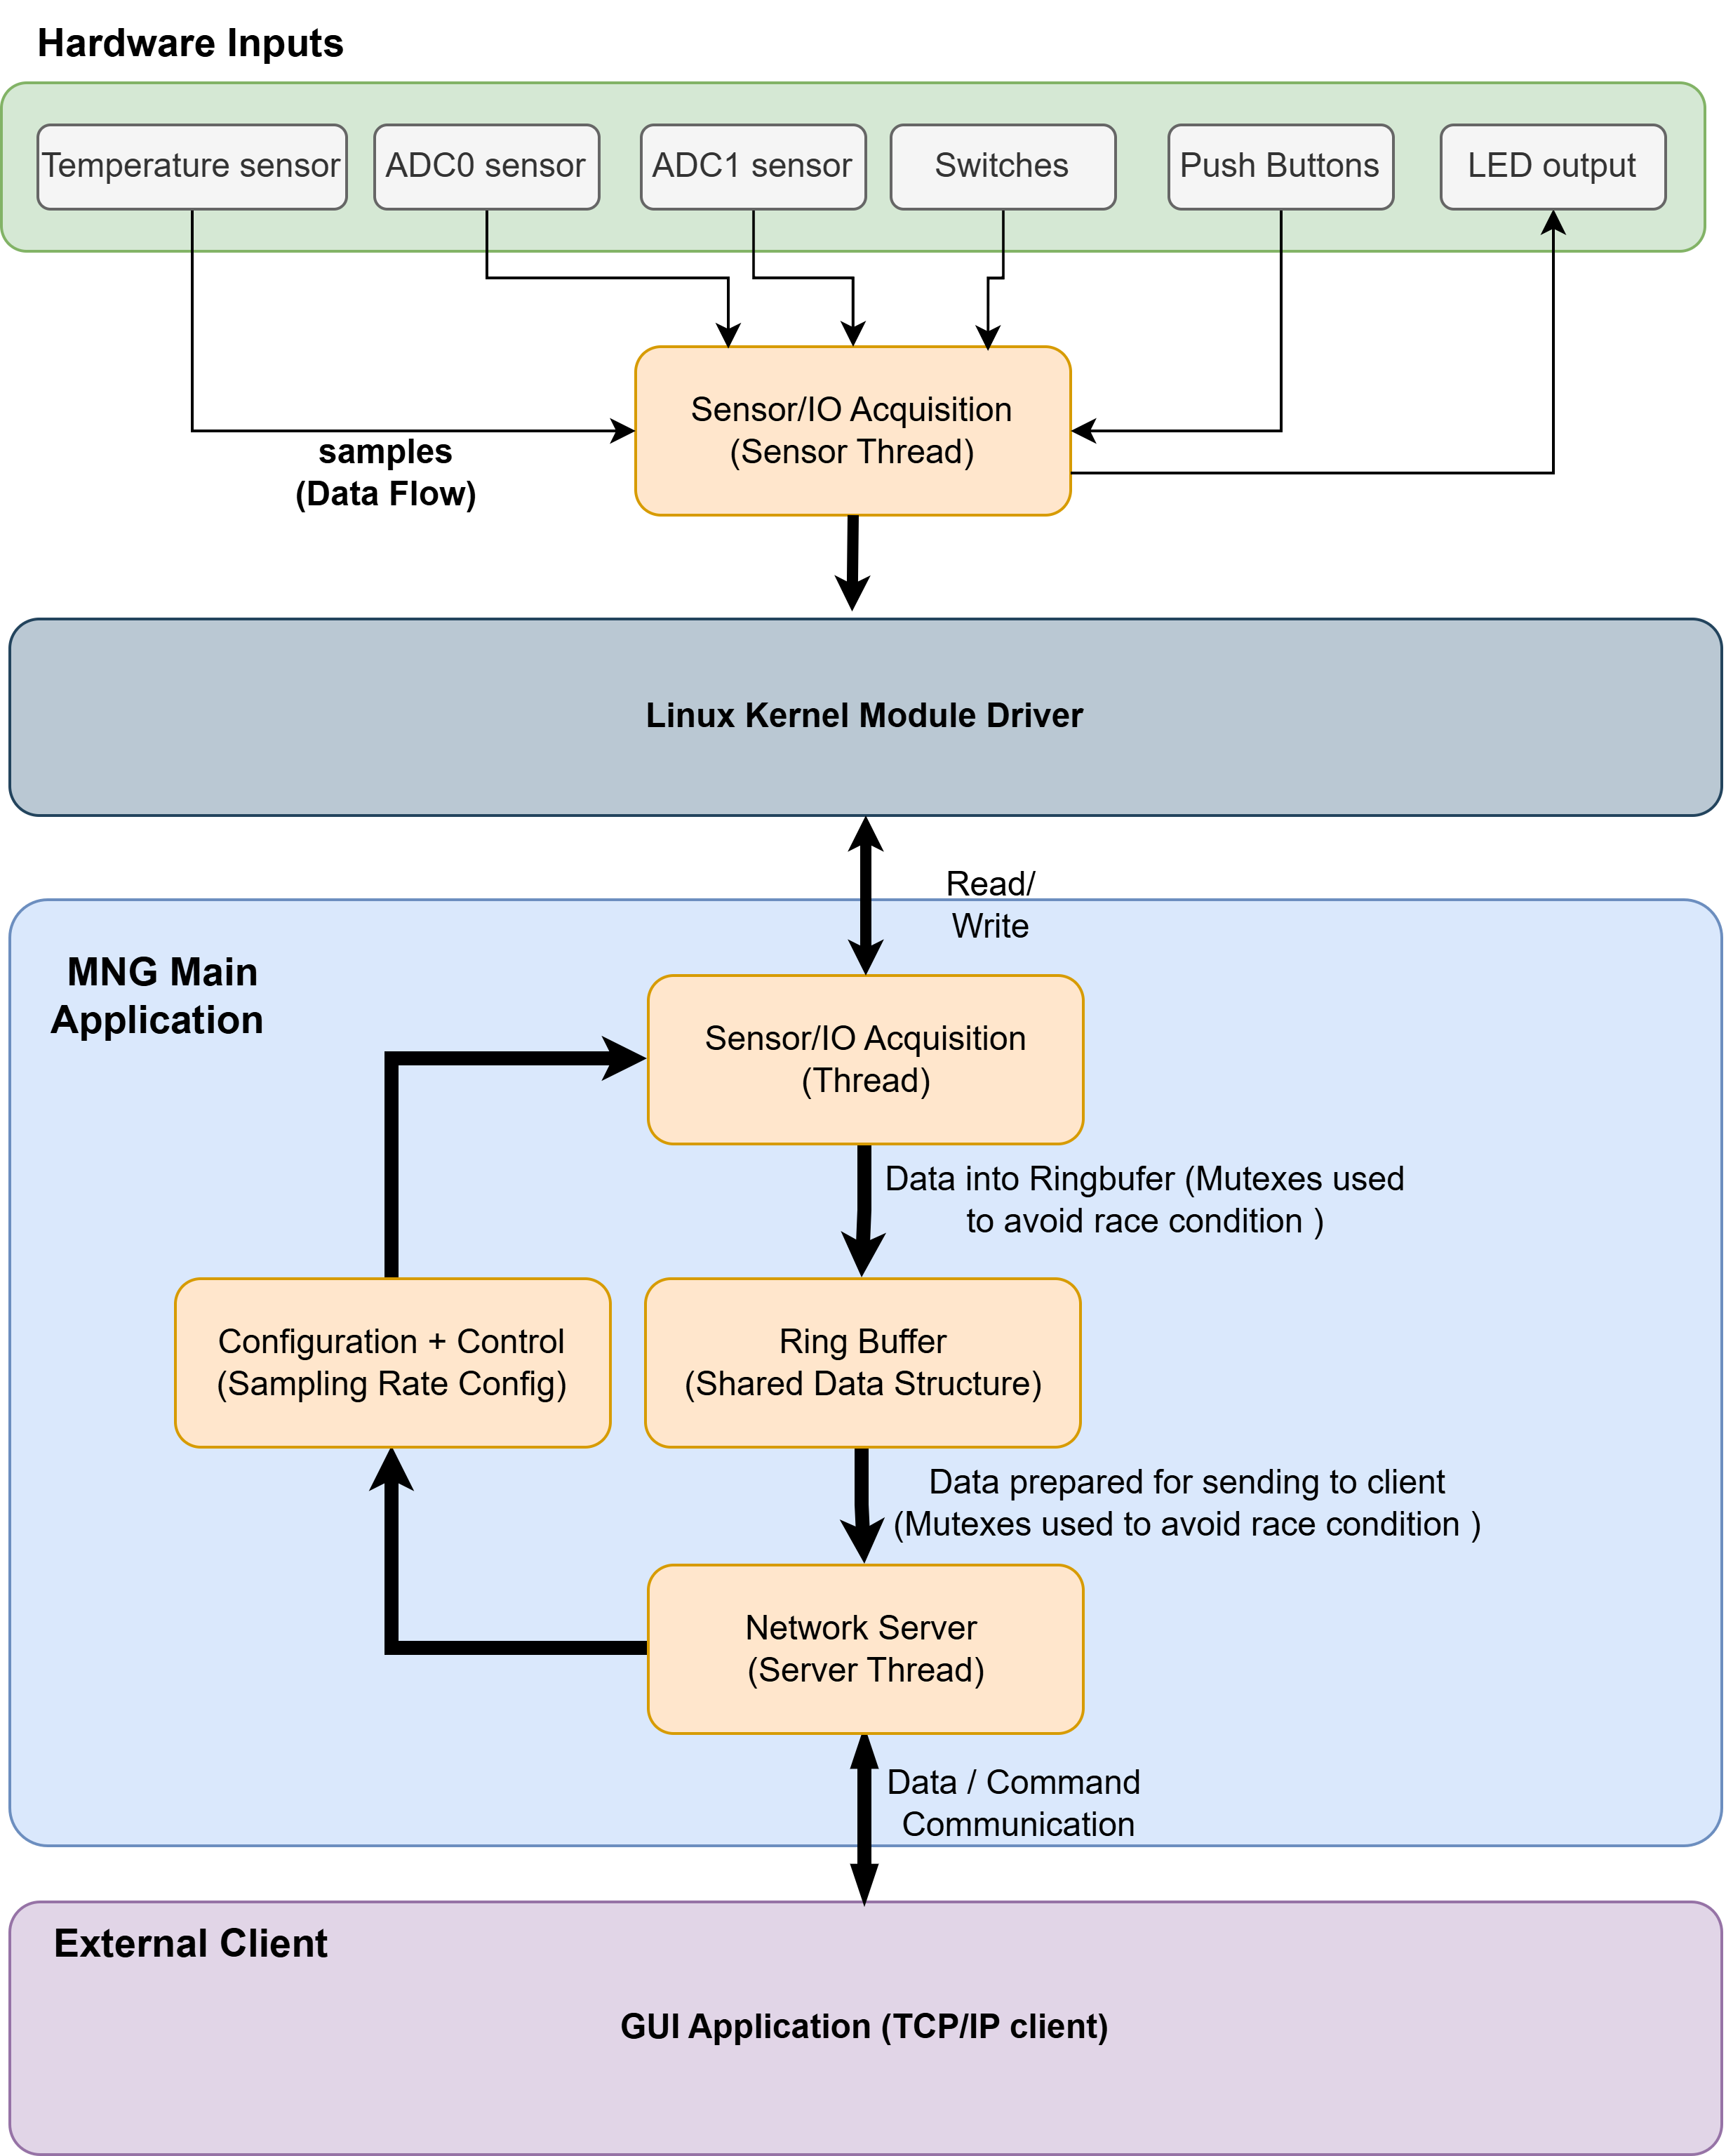
\includegraphics[width = 0.75\textwidth]{media/softArch2.png}
	\caption{Software Architecture of the Measurement Network Gateway}
	\label{fig-softArch}
\end{figure}
The Measurement Network Gateway (MNG) software architecture is designed as a layered and modular system running on an embedded Linux platform based on the Zynq architecture. The design separates hardware interaction, kernel-level driver functionality, user-space application logic, and external client communication to ensure scalability, maintainability, and real-time capable data acquisition.

At the lowest level, multiple sensors and digital inputs (temperature sensor, ADC channels, switches, and push buttons) are connected to the hardware, available throught the IP generated in Vivado Design suite in VHDL language. Based on the custom hardware designed, Petalinux is created and for the custom hardware a Linux Kernel Module was developed. This kernel module encapsulates low-level hardware access and exposes a character device interface \texttt{(/dev/meascdd}) to user space.

The MNG main application operates entirely in user space and follows a multi-threaded design. A dedicated sensor acquisition thread periodically reads data from the device interface and stores sampled values into a thread-safe ring buffer. Synchronization mechanisms such as mutexes and condition variables ensure safe concurrent access between threads.

A separate network server thread retrieves data from the ring buffer and transmits it to an external GUI client via a TCP/IP-based custom communication protocol. In addition to data streaming, the server thread processes configuration and control commands received from the client, such as sampling rate adjustments. A configuration manager component updates system parameters accordingly and propagates them to the acquisition layer.

Overall, the architecture provides a structured and scalable framework for reliable sensor acquisition, real-time processing, and network-based monitoring in embedded Linux environments.

\section{Data acquisition and sensor measurement}
The sensor thread is the core data acquisition component of the Measurement Network Gateway, responsible for continuously reading and timestamping data from all connected sensors at configurable sampling rates. Running as a dedicated POSIX thread, it operates independently from the server thread, ensuring that sensor sampling remains uninterrupted regardless of network activity or client communication state.

Upon startup, the thread attempts to open the hardware device file \texttt{/dev/meascdd} for direct sensor access. If the device is unavailable, the thread automatically falls back to simulation mode, generating synthetic sensor data that mimics real hardware behaviour, allowing the system to be tested and demonstrated without physical hardware. Following device initialisation, the temperature sensor is powered up and all timing references are established using a high-resolution elapsed time counter.

The thread manages five independent sensors --- temperature, two ADC channels, a switch bank, and a push button --- each operating at its own configurable sampling frequency. A deadline-based scheduling approach is employed, where each sensor maintains its own next scheduled sample time, and the thread sleeps only until the nearest upcoming deadline. This design minimises CPU usage while preserving timing accuracy across all channels simultaneously.

The following code show the basic structure of the threads created inside the main application. 
\begin{minted}[bgcolor = lightgray, tabsize = 4, breaklines]{c}
typedef struct {
	pthread_t       thobj;
	pthread_cond_t  thcond;
	pthread_mutex_t thmutex;
	config_struct   th_config;
	short int       thkill;
} thread_struct;
\end{minted}

The initial default sampling rate of all the sensors are set to \SI{300}{\hertz} and when the program starts, then it going to sample all the sensor with this frequency, but when connected to client, it can be changed to the desired sampling rate from the user. 

The following code shows the initial sampling rate configuration of all the sensors: 
\begin{minted}[bgcolor = lightgray, tabsize = 4, breaklines]{c}
config_struct main_config = {
.temp_config   = 300,
.adc0_config   = 300,
.adc1_config   = 300,
.switch_config = 300,
.pushb_config  = 300
};
\end{minted}

At the initial stage of the thread function, the thread opens the device file \texttt{/dev/meascdd} to access the hardware sensors. If the device file cannot be opened (e.g., due to missing hardware or permissions), the thread enters a simulation mode where it generates synthetic sensor data for testing purposes. This fallback mechanism ensures that the application can be developed and demonstrated even in the absence of physical hardware and then the ring buffer is initialized to store the acquired sensor data. The thread also powers up the temperature sensor and initializes timing references for accurate timestamping of samples. Alongside the ring-buffer initialization, the thread also initializes the timer used for timestamping the acquired samples. This timer is typically implemented using a high-resolution clock source (e.g., \texttt{clock\_gettime()} with \texttt{CLOCK\_MONOTONIC}) to provide microsecond precision timestamps for each sensor reading.

Then it check the sampling rates for each sensor and if the sampling rate is zero, then it will not sample that sensor and it will just sleep until the next deadline of the sensors that have non-zero sampling rates. This design allows for dynamic enabling/disabling of individual sensors without affecting the overall thread operation.

Since each sensor should be sampled independently at its own rate, the thread maintains separate timing references for each sensor type. It calculates the next scheduled sample time for each sensor based on the current time and the configured sampling period. The thread then sleeps until the nearest upcoming deadline, ensuring efficient CPU usage while maintaining accurate timing for all sensors. When a sensor's deadline is reached, the thread reads the sensor value from the device file (or generates a simulated value), timestamps it with microsecond precision, and stores it in the shared ring buffer for later retrieval by the server thread. This process continues indefinitely until a termination signal is received.

Due to the requirement of the project that push-buttons and switches shall be used as an auxilary digital inputs, the state of the switches are used to set the LEDs on the ZedBoard. For example, when the first switch is turned on, the first LED will be turned on and when the second switch is turned on, the second LED will be turned on and so on. This provides a simple visual feedback mechanism for the state of the switches.

The following code shows the device file opening, ring-buffer initialization, timer initialization and the MAX31865 temperature sensor power-up: 
\begin{minted}[bgcolor = lightgray, tabsize = 4, breaklines]{c}
	int fd = open("/dev/meascdd", O_RDWR);
    if (fd < 0) {
        simulation = 1;
        printf("Device open failed - simulation mode\n");
    } else {
        printf("Device opened successfully\n");
    }

    InitTimer();
    InitRingBuffer();
\end{minted}

The following code shows the sampling period calculation with zero rate handling. If the user wants to disable reading one of the sensors, then he can set the sampling rate of that sensor to zero and then the thread will not sample that sensor and it will just sleep until the next deadline of the sensors that have non-zero sampling rates. 
\begin{minted}[bgcolor = lightgray, tabsize = 4, breaklines]{c}
	// Get initial timestamps for all sensors
	uint64_t next_temp_time   = GetElapsedTime();
	uint64_t next_adc0_time   = GetElapsedTime();
	uint64_t next_adc1_time   = GetElapsedTime();
	uint64_t next_switch_time = GetElapsedTime();
	uint64_t next_pushb_time  = GetElapsedTime();

	// Calculate sampling periods with zero-rate protection
	uint64_t period_temp_us   = (main_config.temp_config > 0) ? 
								1000000ULL / main_config.temp_config : 0;
	uint64_t period_adc0_us   = (main_config.adc0_config > 0) ? 
								1000000ULL / main_config.adc0_config : 0;
	uint64_t period_adc1_us   = (main_config.adc1_config > 0) ? 
								1000000ULL / main_config.adc1_config : 0;
	uint64_t period_switch_us = (main_config.switch_config > 0) ? 
								1000000ULL / main_config.switch_config : 0;
	uint64_t period_pushb_us  = (main_config.pushb_config > 0) ? 
								1000000ULL / main_config.pushb_config : 0;

	// Track enabled sensors based on non-zero rates
	int temp_enabled   = (main_config.temp_config > 0);
	int adc0_enabled   = (main_config.adc0_config > 0);
	int adc1_enabled   = (main_config.adc1_config > 0);
	int switch_enabled = (main_config.switch_config > 0);
	int pushb_enabled  = (main_config.pushb_config > 0);
\end{minted}

\subsection{Main Sampling Loop Implementation}

The core of the sensor data acquisition system is implemented as an infinite loop that executes a deadline-driven scheduling algorithm for all five sensor types. At the beginning of each iteration, the thread checks for termination signals by examining both the thread-specific kill flag and the global shutdown flag under mutex protection, ensuring safe and coordinated thread termination. The loop then retrieves the current high-resolution timestamp using the \texttt{GetElapsedTime()} function and calculates the nearest upcoming sampling deadline by comparing the next scheduled sampling times of all enabled sensors, selecting the smallest value as the sleep target. A critical safety check handles the scenario where all sensors are disabled (i.e., all sampling rates set to zero), causing the sleep target to remain at \texttt{UINT64\_MAX}; in this case, the thread enters a 10-millisecond sleep before re-evaluating, preventing CPU exhaustion while remaining responsive to shutdown signals. 

When sensors are enabled and the current time precedes the nearest deadline, the thread performs a granular sleep operation, breaking the sleep into small chunks of maximum 100 microseconds. This chunked approach maintains system responsiveness by allowing early wake-up on shutdown signals and enabling timely detection of configuration changes. After waking, the loop sequentially evaluates each enabled sensor to determine if its sampling deadline has been reached; for those that have, the appropriate hardware read or simulation function is invoked, the sampled value is timestamped and pushed to the ring buffer via \texttt{PushRB()}, and the next sampling time is advanced by the configured period. 

Of particular note is the switch-handling logic, which implements a visual feedback mechanism by comparing the current switch state against the last known state stored in a static variable. Only when a state change is detected are the LEDs updated via \texttt{LedWrite()}, ensuring efficient operation by avoiding redundant writes while providing immediate visual confirmation of input state changes. This direct mapping between switch positions and LEDs (switch N controls LED N) offers intuitive feedback without requiring additional software monitoring. The overall architecture ensures precise, jitter-minimized sampling intervals while maintaining system responsiveness and proper synchronization between hardware inputs and visual outputs.
\begin{minted}[bgcolor = lightgray, tabsize = 4, breaklines]{c}
while (1)
{
    // Check for thread termination
    pthread_mutex_lock(&sensor_thread.thmutex);
    int kill = sensor_thread.thkill;
    pthread_mutex_unlock(&sensor_thread.thmutex);
    if (kill || g_shutdown) break;
    
    uint64_t current_time = GetElapsedTime();
    
    // Calculate the nearest upcoming sampling deadline
    uint64_t sleep_target = UINT64_MAX;
    
    if (temp_enabled && next_temp_time < sleep_target) 
        sleep_target = next_temp_time;
    if (adc0_enabled && next_adc0_time < sleep_target) 
        sleep_target = next_adc0_time;
    if (adc1_enabled && next_adc1_time < sleep_target) 
        sleep_target = next_adc1_time;
    if (switch_enabled && next_switch_time < sleep_target) 
        sleep_target = next_switch_time;
    if (pushb_enabled && next_pushb_time < sleep_target) 
        sleep_target = next_pushb_time;
    
    // Handle all-sensors-disabled case
    if (sleep_target == UINT64_MAX) {
        usleep(10000);  // Sleep 10ms and check again
        continue;
    }
    
    // Sleep until the next sampling deadline
    if (current_time < sleep_target) {
        uint64_t sleep_us = sleep_target - current_time;
        while (sleep_us > 0) {
            uint64_t chunk = (sleep_us > 100) ? 100 : sleep_us;
            usleep(chunk);
            sleep_us -= chunk;
            current_time = GetElapsedTime();
            if (current_time >= sleep_target) break;
            if (g_shutdown) break;
        }
    }
    
    if (g_shutdown) break;
    
    // Sample each enabled sensor if its deadline has arrived
    if (temp_enabled && current_time >= next_temp_time) {
        // Read temperature sensor
        int raw = 0;
        if (simulation) {
            raw = (int)(GenerateFakeTemperature(current_time) * 100);
        } else {
            TempRead(fd, &raw);
        }
        PushRB(sid_temp, current_time, (uint32_t)raw);
        next_temp_time += period_temp_us;
    }
    
    // Similar blocks for ADC0, ADC1, switches, and push-buttons...
    
    // Switch-LED feedback mechanism
    if (switch_enabled && current_time >= next_switch_time) {
        uint8_t sw = ReadSwitch(fd);
        static uint8_t LastSwitchState = 0xff;
        
        // Update LEDs only when switch state changes
        if (sw != LastSwitchState) {
            LedWrite(fd, sw);  // Direct mapping: switch N -> LED N
            LastSwitchState = sw;
        }
        PushRB(sid_switches, current_time, sw);
        next_switch_time += period_switch_us;
    }
}
\end{minted}

























\section{Network server implementation}
The Measurement Network Gateway requires a robust communication mechanism to enable remote access to sensor data and configuration control. To fulfill this requirement, a TCP/IP-based server has been implemented as an integral component of the main application. This section presents the design, implementation, and operational characteristics of the network server subsystem.

\subsection{TCP/IP Server Fundamentals}

The Transmission Control Protocol (TCP) is a connection-oriented, reliable transport layer protocol that operates on top of the Internet Protocol (IP). Unlike the User Datagram Protocol (UDP), which provides best-effort delivery, TCP guarantees ordered and error-free delivery of data through mechanisms such as acknowledgments, retransmissions, and flow control. The TCP/IP socket programming interface provides a standardized API for implementing network communication in userspace applications.

A typical TCP server follows a well-defined operational sequence: socket creation, binding to a specific IP address and port, listening for incoming connections, accepting client connections, and finally exchanging data through send and receive operations. This client-server model forms the foundation of most networked applications, from web servers to industrial monitoring systems.

\subsection{Design Rationale for TCP in MNG}

For the Measurement Network Gateway application, TCP was selected over UDP for several critical reasons. First, the reliable delivery guarantee ensures that configuration commands (such as sampling rate updates) and sensor data reach the client without loss or corruption, which is essential for accurate monitoring and control. Second, the connection-oriented nature of TCP provides clear session management, allowing the server to track client connection status and handle disconnections gracefully. Third, the ordered delivery property ensures that timestamped sensor samples arrive in the correct sequence, simplifying client-side processing and visualization.

\subsection{Server Role in the MNG System}

The network server thread acts as the primary interface between the embedded measurement system and external monitoring clients. Its responsibilities include:

\begin{itemize}
	\item Accepting and managing TCP connections from GUI clients and other monitoring tools
	\item Receiving and parsing text-based commands for configuration and control
	\item Retrieving sensor data from the shared ring buffer and transmitting it to connected clients
	\item Coordinating with the sensor acquisition thread through shared configuration structures
	\item Handling connection errors, client disconnections, and graceful shutdown sequences
\end{itemize}

The server operates as an independent pthread within the main application, enabling concurrent sensor acquisition and network communication. Thread-safe access to shared resources (ring buffer and configuration data) is ensured through mutex-based synchronization mechanisms.

\subsection{Server Thread Architecture}
The network server is implemented as a separate POSIX thread (pthread) within the main application, enabling concurrent execution alongside the sensor acquisition thread. This multi-threaded architecture allows the server to handle client communication independently while sensor data continues to be collected in the background without blocking or interference.

The server thread encapsulates all network-related functionality within a single execution context. The thread structure, defined as \texttt{threadstruct} in the main application, contains several essential components:

\begin{itemize}
	\item \texttt{pthread\_t thobj}: The thread object handle used by the pthread library for thread management
	\item \texttt{pthread\_cond\_t thcond}: Condition variable for thread synchronization and signaling
	\item \texttt{pthread\_mutex\_t thmutex}: Mutex for protecting thread-specific shared state
	\item \texttt{config\_struct}: This is the structure used for the sampling rate configuration
	\item \texttt{short int thkill}: Flag for signaling thread termination requests
\end{itemize}

The server thread executes the \texttt{serverthreadfunction()}, which implements the complete TCP server lifecycle from socket initialization through connection handling and graceful shutdown. This function operates in an infinite loop, waiting for and serving client connections until an explicit termination signal is received.

Unlike the sensor thread, which requires configuration parameters to control sampling rates, the server thread operates with a simpler initialization model. Its primary runtime parameters include the TCP port number (defined as \texttt{PORT 50012}) and receive buffer size (\texttt{CMDBUFSIZE 1024} bytes), which are compile-time constants.

To control the data streaming behavior and server operation, a state machine has been implemented using an enumerated type. This state management mechanism allows clients to start, stop, pause, and reconfigure the data stream without disconnecting from the server:

\begin{minted}[bgcolor=lightgray, breaklines, tabsize=4]{c}
	typedef enum {
		STOPPED       = 0,  // Server idle, not streaming data
		RUNNING,            // Actively streaming sensor data to client
		PAUSED,             // Temporarily suspended, maintaining connection
		CONFIGURATION,      // Accepting configuration commands
		DISCONNECT,         // Client-requested disconnect
		SHUTDOWN            // Server shutdown, exit loop entirely
	} stream_state_t;
\end{minted}

Each state represents a distinct operational mode:

\begin{itemize}
	\item \textbf{STOPPED:} The initial state after client connection. The server is connected but not actively transmitting sensor data. It waits for client commands to transition to other states.
	
	\item \textbf{RUNNING:} The server actively retrieves samples from the ring buffer and transmits them to the client. Data streaming continues until a pause, stop, or disconnect command is received.
	
	\item \textbf{PAUSED:} Data streaming is temporarily suspended while maintaining the TCP connection. This allows clients to halt data flow temporarily without losing connection state, useful for GUI operations or processing delays.
	
	\item \textbf{CONFIGURATION:} The server enters a configuration mode where it accepts and processes parameter update commands (e.g., sampling rate changes) without streaming data. This state ensures configuration updates are applied atomically without interfering with data transmission.
	
	\item \textbf{DISCONNECT:} Signals that the client has requested disconnection. The server performs cleanup operations, closes the client socket, and returns to waiting for new connections.
	
	\item \textbf{SHUTDOWN:} Indicates a complete server shutdown request. Unlike DISCONNECT, which only closes the current client connection, SHUTDOWN causes the server thread to exit its main loop entirely, terminating the thread.
\end{itemize}

The server maintains a \texttt{stream\_state\_t} variable that tracks the current state. Client commands trigger state transitions, and the server's behavior in the main loop depends on the current state. This design provides a clean separation between connection management, configuration, and data streaming operations.

The following code shows the structure of each thread created inside the main application: 
\begin{minted}[bgcolor= lightgray, breaklines, tabsize=4]{c}
	typedef struct {
		pthread_t       thobj;
		pthread_cond_t  thcond;
		pthread_mutex_t thmutex;
		config_struct   th_config;
		short int       thkill;
	} thread_struct;
\end{minted}

After definition of the structure of the thread, the server thread can be defined as follows: 

\begin{minted}[bgcolor= lightgray, breaklines, tabsize=4]{c}
thread_struct server_thread;
\end{minted}

\subsubsection{Data Packet Structure}

Sensor data is transmitted to clients using a well-defined binary packet structure. Each packet encapsulates a single sensor sample with its associated metadata:

\begin{minted}[bgcolor=lightgray, breaklines, tabsize=4]{c}
	typedef struct {
		int      sid;      // Sensor ID (1=Temp, 2=ADC0, 3=ADC1, 
						   // 4=Switch, 5=Push-button)
		int      svalue;   // Sensor value (raw reading)
		uint64_t ts;       // Timestamp in microseconds since startup
	} packet;
\end{minted}

This structure, defined as \texttt{packet}, contains three fields totaling 16 bytes (assuming 32-bit integers and 64-bit timestamp on the target platform):

\begin{itemize}
	\item \textbf{sid (Sensor ID):} Identifies which sensor produced the measurement. The sensor ID mapping corresponds to the ring buffer organization: 1 for temperature, 2 for ADC0, 3 for ADC1, 4 for switches, and 5 for push-buttons.
	\item \textbf{svalue (Sensor Value):} The raw sensor reading as retrieved from the hardware. The interpretation of this value depends on the sensor type.
	\item \textbf{ts (Timestamp):} A 64-bit unsigned integer representing microseconds elapsed since the system timer initialization, providing high-precision timing information for each sample.
\end{itemize}


\subsection{Sampling Rate Configuration}
The sensor sampling rates are stored in a shared configuration structure accessible to both the sensor thread (consumer) and the server thread (modifier). To ensure thread-safe access, dedicated functions have been implemented for reading and writing configuration parameters.

\textbf{Configuration Update Function:}

The \texttt{set\_config()} function provides a thread-safe mechanism for updating sampling rate parameters:

\begin{minted}[bgcolor=lightgray, breaklines, tabsize=4]{c}
	void set_config(config_struct *config)
	{
		pthread_mutex_lock(&server_thread.thmutex);
		main_config.temp_config   = config->temp_config;
		main_config.adc0_config   = config->adc0_config;
		main_config.adc1_config   = config->adc1_config;
		main_config.switch_config = config->switch_config;
		main_config.pushb_config  = config->pushb_config;
		pthread_mutex_unlock(&server_thread.thmutex);
	}
\end{minted}

This function accepts a pointer to a \texttt{config\_struct} containing the new sampling rate values (in microseconds) for each sensor type. The entire update operation is protected by the server thread's mutex (\texttt{server\_thread.thmutex}) to prevent race conditions when the sensor thread is reading these values. By locking the mutex, the function guarantees atomic updates of all five configuration parameters, ensuring the sensor thread never observes a partially-updated configuration state.

\textbf{Configuration Display Function:}

For debugging and verification purposes, the \texttt{print\_config()} function outputs the current configuration to the console:

\begin{minted}[bgcolor=lightgray, breaklines, tabsize=4]{c}
	void print_config(void)
	{
		printf("temp_config:     %u\n", main_config.temp_config);
		printf("adc0_config:     %u\n", main_config.adc0_config);
		printf("adc1_config:     %u\n", main_config.adc1_config);
		printf("switches_config: %u\n", main_config.switch_config);
		printf("pushb_config:    %u\n", main_config.pushb_config);
	}
\end{minted}

This function prints all sampling period values in microseconds. While not mutex-protected (as it's a read-only operation for display purposes), it provides valuable runtime visibility into the current system configuration.

When a client sends a configuration command over the network, the server thread parses the command, extracts the new sampling rate values, populates a \texttt{config\_struct}, and calls \texttt{set\_config()} to apply the changes. The sensor thread, which continuously checks the \texttt{main\_config} structure in its acquisition loop, automatically adopts the new sampling rates for subsequent sensor reads without requiring a restart.

This design enables dynamic runtime reconfiguration of the measurement system, allowing clients to optimize sampling rates based on real-time requirements or system load conditions.

%start of the server thread function 


\subsection{TCP Socket Implementation}

\subsubsection{Thread Function Initialization}

The server thread function begins execution by initializing essential variables and data structures required for network communication and data transmission. This initialization phase prepares all necessary resources before socket creation:

\begin{minted}[bgcolor=lightgray, breaklines, tabsize=4]{c}
	void *server_thread_function(void *arg)
	{
		(void)arg;  // Unused parameter
		packet payload[96];
		char   receive_command[CMD_BUF_SIZE];
		
		struct sockaddr_in server_address, client_addr;
		socklen_t client_addr_len = sizeof(client_addr);
		
		stream_state = PAUSED;
		// ... continue with socket creation
	}
\end{minted}

\textbf{Function Parameter:}

The function signature follows the POSIX pthread convention, accepting a \texttt{void *arg} parameter that can be used to pass initialization data to the thread. In this implementation, no configuration parameters are required by the server thread, so the argument is explicitly cast to \texttt{(void)arg} to suppress compiler warnings about unused parameters.

\textbf{Data Transmission Buffer:}

\begin{minted}[bgcolor=lightgray, breaklines, tabsize=4]{c}
	packet payload[96];
\end{minted}

A fixed-size array of 96 \texttt{packet} structures is allocated on the stack for batch data transmission. Each \texttt{packet} contains sensor ID, timestamp, and value fields (16 bytes total), resulting in a payload buffer of \texttt{1536 bytes (1.5 KB)}. This size represents a trade-off between:

\begin{itemize}
	\item Memory consumption on the embedded platform
	\item Network transmission efficiency (larger batches reduce per-packet overhead)
	\item Response latency (smaller batches provide faster initial response)
\end{itemize}

The value of 96 was chosen empirically to provide efficient bulk data transfer while remaining within reasonable stack memory limits.

\textbf{Command Reception Buffer:}

\begin{minted}[bgcolor=lightgray, breaklines, tabsize=4]{c}
	char receive_command[CMD_BUF_SIZE];
\end{minted}

A character buffer of size \texttt{CMD\_BUF\_SIZE} (1024 bytes) is allocated for receiving text-based commands from clients. This size is sufficient for all supported commands, including the \texttt{configure} command which contains five unsigned integer values plus the command keyword.

\textbf{Socket Address Structures:}

\begin{minted}[bgcolor=lightgray, breaklines, tabsize=4]{c}
	struct sockaddr_in server_address, client_addr;
	socklen_t client_addr_len = sizeof(client_addr);
\end{minted}

Two \texttt{sockaddr\_in} structures are declared:
\begin{itemize}
	\item \texttt{server\_address}: Stores the server's binding address (IP and port)
	\item \texttt{client\_addr}: Populated by \texttt{accept()} with the connecting client's address information
\end{itemize}

The \texttt{client\_addr\_len} variable holds the size of the client address structure, required by the \texttt{accept()} system call.

\textbf{Initial Stream State:}

\begin{minted}[bgcolor=lightgray, breaklines, tabsize=4]{c}
	stream_state = PAUSED;
\end{minted}

The global stream state is explicitly set to \texttt{PAUSED} at thread startup. This ensures that when a client connects, the server does not immediately begin streaming data. Instead, it waits for explicit commands from the client (such as \texttt{start}) before transmitting sensor samples. This design provides the client with full control over data flow timing.

Following these initialization steps, the server proceeds to create and configure the listening socket.

\subsubsection{Socket Creation and Configuration}
Upon thread startup, the server thread function begins by creating a TCP socket and configuring it for proper operation. The socket is created using the standard POSIX socket API:

\begin{minted}[bgcolor=lightgray, breaklines, tabsize=4]{c}
	int server_sock = socket(AF_INET, SOCK_STREAM, 0);
	if (server_sock < 0) { 
		perror("socket"); 
		return NULL; 
	}
\end{minted}
The \texttt{socket()} function is called with three arguments:
\begin{itemize}
	\item \texttt{AF\_INET}: Specifies the IPv4 address family
	\item \texttt{SOCK\_STREAM}: Indicates a TCP connection-oriented socket (as opposed to \texttt{SOCK\_DGRAM} for UDP)
	\item \texttt{0}: Lets the system choose the appropriate protocol (TCP for stream sockets)
\end{itemize}

If socket creation fails (returns a negative value), an error message is printed and the thread terminates, preventing further execution with an invalid socket descriptor.

Following socket creation, the \texttt{SO\_REUSEADDR} socket option is enabled:

\begin{minted}[bgcolor=lightgray, breaklines, tabsize=4]{c}
	int opt = 1;
	setsockopt(server_sock, SOL_SOCKET, SO_REUSEADDR, 
	&opt, sizeof(opt));
\end{minted}

This option is critical during development and testing. By default, when a TCP server closes, the operating system keeps the port in a TIME\_WAIT state for several minutes to ensure all delayed packets are properly handled. The \texttt{SO\_REUSEADDR} option allows immediate rebinding to the same port after server restart, preventing "Address already in use" errors. This is particularly useful when repeatedly testing and restarting the server during development without having to wait for the TIME\_WAIT period to expire.


\subsubsection{Address Binding and Port Assignment}

After socket creation and configuration, the server must bind the socket to a specific network address and port number. This process associates the socket with a particular interface and port that clients will use to connect.

The server address structure is initialized and populated:

\begin{minted}[bgcolor=lightgray, breaklines, tabsize=4]{c}
	struct sockaddr_in server_address;
	
	memset(&server_address, 0, sizeof(server_address));
	server_address.sin_family      = AF_INET;
	server_address.sin_addr.s_addr = INADDR_ANY;
	server_address.sin_port        = htons(PORT);
\end{minted}

The \texttt{sockaddr\_in} structure contains three key fields:

\begin{itemize}
	\item \textbf{sin\_family}: Set to \texttt{AF\_INET} to match the socket's address family (IPv4)
	\item \textbf{sin\_addr.s\_addr}: Set to \texttt{INADDR\_ANY} (0.0.0.0), which instructs the server to listen on all available network interfaces. This means the server accepts connections from any interface, whether Ethernet, loopback (127.0.0.1), or any other configured network adapter on the ZedBoard
	\item \textbf{sin\_port}: Set to port 50012 (defined by the \texttt{PORT} constant) using \texttt{htons()} to convert from host byte order to network byte order (big-endian)
\end{itemize}

The binding operation associates this address information with the socket:

\begin{minted}[bgcolor=lightgray, breaklines, tabsize=4]{c}
	if (bind(server_sock, (struct sockaddr *)&server_address,
	sizeof(server_address)) < 0) {
		perror("bind"); 
		close(server_sock); 
		return NULL;
	}
\end{minted}

If binding fails (e.g., the port is already in use by another process, or insufficient permissions), the error is logged, the socket is closed to release resources, and the thread terminates. Port 50012 was selected as it falls within the dynamic/private port range (49152-65535), avoiding conflicts with well-known services and reducing the likelihood of permission issues.

\subsubsection{Listen Mode and Connection Queue}

After successful binding, the socket must be placed in listening mode to accept incoming client connections. This is accomplished with the \texttt{listen()} system call:

\begin{minted}[bgcolor=lightgray, breaklines, tabsize=4]{c}
	if (listen(server_sock, 1) < 0) {
		perror("listen"); 
		close(server_sock); 
		return NULL;
	}
\end{minted}

The \texttt{listen()} function takes two parameters:
\begin{itemize}
	\item \textbf{server\_sock}: The bound socket descriptor
	\item \textbf{backlog (1)}: The maximum length of the queue for pending connections
\end{itemize}

The backlog parameter is set to 1, which means the operating system will queue at most one pending connection request. This value is consistent with the server's single-client sequential architecture. When a client is already connected and being served, any additional connection attempts are either queued (if the queue is empty) or rejected (if the queue is full).

In practice, with a backlog of 1:
\begin{itemize}
	\item If no client is connected, the first connection attempt succeeds immediately
	\item If one client is connected and actively being served, a second connection attempt may be queued
	\item A third connection attempt will likely be rejected by the operating system
\end{itemize}

After successful \texttt{listen()}, the socket is ready to accept connections. The server also publishes the server socket descriptor to a global variable for potential access by the shutdown handler:

\begin{minted}[bgcolor=lightgray, breaklines, tabsize=4]{c}
	pthread_mutex_lock(&g_socket_lock);
	g_server_socket = server_sock;
	pthread_mutex_unlock(&g_socket_lock);
	
	printf("Server listening on port %d\n", PORT);
\end{minted}

This mutex-protected assignment ensures thread-safe access to the socket descriptor, which is important if the shutdown mechanism needs to forcibly close the socket from another execution context.

\subsubsection{Client Connection Acceptance}

With the server socket in listening mode, the outer loop of the server thread function continuously waits for incoming client connections using the \texttt{accept()} system call:

\begin{minted}[bgcolor=lightgray, breaklines, tabsize=4]{c}
	while (!g_shutdown)
	{
		printf("Waiting for client...\n");
		
		int client_sock = accept(server_sock,
		(struct sockaddr *)&client_addr,
		&client_addr_len);
		if (client_sock < 0) {
			if (g_shutdown) break;
			perror("accept");
			continue;
		}
		
		printf("Client connected\n");
		// ... proceed to serve client
	}
\end{minted}

The \texttt{accept()} call is a blocking operation that suspends the thread until a client initiates a connection. When a connection request arrives, \texttt{accept()} performs the TCP three-way handshake, establishes the connection, and returns a new socket descriptor (\texttt{client\_sock}) dedicated to communication with that specific client.

Key aspects of the acceptance process:

\begin{itemize}
	\item \textbf{Blocking behavior}: The thread remains blocked at \texttt{accept()} until a client connects or the socket is closed
	\item \textbf{Client information}: The \texttt{client\_addr} structure is populated with the client's IP address and port number, though this information is not currently used for access control or logging
	\item \textbf{Error handling}: If \texttt{accept()} fails, the server checks whether failure was due to shutdown (socket closed intentionally); otherwise, it logs the error and continues waiting for the next connection attempt
	\item \textbf{Sequential service}: Once a client is accepted, the server enters the inner loop to serve that client exclusively until disconnection
\end{itemize}

After accepting a connection, the client socket descriptor is published to a global variable for potential access during shutdown:

\begin{minted}[bgcolor=lightgray, breaklines, tabsize=4]{c}
	pthread_mutex_lock(&g_socket_lock);
	g_client_socket = client_sock;
	pthread_mutex_unlock(&g_socket_lock);
\end{minted}

The stream state is also reset to \texttt{PAUSED}, ensuring the server starts in a known state where it awaits commands without automatically streaming data.


\subsection{Client Connection Management}

\subsubsection{Single-Client Connection Model}

The server implements a **sequential single-client architecture**, meaning it serves only one client at a time. This design is reflected in both the socket configuration (listen backlog of 1) and the dual-loop structure of the server thread function.

The outer loop continuously accepts new client connections in sequence:

\begin{minted}[bgcolor=lightgray, breaklines, tabsize=4]{c}
	while (!g_shutdown)
	{
		printf("Waiting for client...\n");
		
		int client_sock = accept(server_sock,
		(struct sockaddr *)&client_addr,
		&client_addr_len);
		// ... serve client in inner loop
	}
\end{minted}

This architecture provides several advantages for the MNG application:

\begin{itemize}
	\item \textbf{Simplified resource management}: A single client eliminates the need for complex per-client state management and thread pools
	\item \textbf{Predictable data flow}: The ring buffer has only one consumer (the server serving one client), simplifying synchronization
	\item \textbf{Deterministic behavior}: System performance and response times are consistent and easy to debug
	\item \textbf{Application requirements}: The primary use case is a single GUI client monitoring the gateway; multiple simultaneous clients are not required
	\item \textbf{Resource constraints}: The embedded ZedBoard platform has limited processing power and memory; serving multiple concurrent clients would increase CPU load and complicate buffer management
\end{itemize}

When a client is connected and being served, any additional connection attempts must wait until the current client disconnects. The server does not support concurrent multi-client connections.

\subsubsection{Connection Establishment}

The outer loop implements the connection acceptance and sequential client handling logic. After successfully entering listening mode, the server enters a continuous loop that waits for and serves clients one at a time:

\begin{minted}[bgcolor=lightgray, breaklines, tabsize=4]{c}
	while (!g_shutdown)
	{
		printf("Waiting for client...\n");
		
		int client_sock = accept(server_sock,
		(struct sockaddr *)&client_addr,
		&client_addr_len);
		if (client_sock < 0) {
			if (g_shutdown) break;
			perror("accept");
			continue;
		}
		
		/* Publish client fd */
		pthread_mutex_lock(&g_socket_lock);
		g_client_socket = client_sock;
		pthread_mutex_unlock(&g_socket_lock);
		
		printf("Client connected\n");
		stream_state = PAUSED;
		
		/* ---- INNER LOOP: serve one client ---- */
		// ... command processing loop
	}
\end{minted}

\textbf{Blocking Accept:}

The \texttt{accept()} call is a blocking operation that suspends the server thread until a client initiates a TCP connection. During this time, the thread consumes no CPU resources. When a connection request arrives, the operating system completes the TCP three-way handshake and \texttt{accept()} returns a new socket descriptor (\texttt{client\_sock}) dedicated to communication with that specific client.

\textbf{Error Handling:}

If \texttt{accept()} returns a negative value, indicating an error, the server performs two checks:

\begin{enumerate}
	\item \textbf{Shutdown check}: If \texttt{g\_shutdown} is set, the error is expected (the listening socket was closed intentionally by \texttt{request\_shutdown()}), and the loop exits cleanly with \texttt{break}
	\item \textbf{Other errors}: If not a shutdown scenario, the error is logged with \texttt{perror()}, and the loop continues with \texttt{continue}, returning to wait for the next connection attempt
\end{enumerate}

This error handling ensures the server remains robust against transient network errors while responding appropriately to intentional shutdown requests.

\textbf{Client Socket Registration:}

Upon successful connection acceptance, the client socket descriptor is stored in the global variable \texttt{g\_client\_socket} within a mutex-protected critical section:

\begin{minted}[bgcolor=lightgray, breaklines, tabsize=4]{c}
	pthread_mutex_lock(&g_socket_lock);
	g_client_socket = client_sock;
	pthread_mutex_unlock(&g_socket_lock);
\end{minted}

This registration serves two purposes:
\begin{itemize}
	\item Allows the \texttt{request\_shutdown()} function to access and close the client socket from a different execution context
	\item Provides thread-safe access to the socket descriptor for potential monitoring or diagnostic purposes
\end{itemize}

\textbf{Initial State Configuration:}

After registering the client socket, the stream state is reset to \texttt{PAUSED}:

\begin{minted}[bgcolor=lightgray, breaklines, tabsize=4]{c}
	stream_state = PAUSED;
\end{minted}

This ensures each newly connected client starts in a known state where the server awaits commands without automatically streaming data. The client must explicitly issue a \texttt{start} command to begin receiving sensor data, providing full control over data flow timing.

Following these initialization steps, execution proceeds to the inner loop where the server receives and processes commands from the connected client.

\subsubsection{Disconnect Handling and Cleanup}

Client disconnection can occur through three mechanisms: graceful client-initiated disconnect, explicit disconnect command, or connection failure. The server handles all scenarios and performs appropriate cleanup before returning to the outer loop to await the next client.

\textbf{Normal Disconnection:}

When \texttt{recv()} returns 0 in the inner loop, it indicates the client closed the connection gracefully (TCP FIN received). The inner loop exits with \texttt{break}, and execution continues in the outer loop's cleanup section:

\begin{minted}[bgcolor=lightgray, breaklines, tabsize=4]{c}
	/* Clean up client socket if not already closed */
	pthread_mutex_lock(&g_socket_lock);
	if (g_client_socket >= 0) {
		close(g_client_socket);
		g_client_socket = -1;
	}
	pthread_mutex_unlock(&g_socket_lock);
\end{minted}

\textbf{Command-Initiated Disconnect:}

When the client sends a \texttt{disconnect} command, the stream state is set to \texttt{DISCONNECT}, triggering the following cleanup sequence in the inner loop:

\begin{minted}[bgcolor=lightgray, breaklines, tabsize=4]{c}
	if (stream_state == DISCONNECT) {
		printf("Closing client connection\n");
		shutdown(client_sock, SHUT_RDWR);
		close(client_sock);
		
		pthread_mutex_lock(&g_socket_lock);
		g_client_socket = -1;
		pthread_mutex_unlock(&g_socket_lock);
		break;  /* go back to accept() */
	}
\end{minted}

The \texttt{shutdown()} call with \texttt{SHUT\_RDWR} disables both send and receive operations on the socket, informing the peer of the intentional closure. The socket is then closed with \texttt{close()}, releasing system resources. The global client socket variable is reset to -1 (invalid descriptor) to indicate no client is connected.

\textbf{Return to Accept Loop:}

After cleanup, the inner loop exits with \texttt{break}, returning execution to the outer loop's \texttt{accept()} call. The server is now ready to accept a new client connection, completing the sequential client service cycle.

This architecture ensures clean resource management and allows the server to serve multiple clients sequentially over its lifetime without requiring restart.


\subsection{Command Protocol and Communication}

\subsubsection{Command Receive Loop Implementation}

The inner loop continuously monitors for incoming commands from the connected client using non-blocking I/O:

\begin{minted}[bgcolor=lightgray, breaklines, tabsize=4]{c}
	while (!g_shutdown)
	{
		memset(receive_command, 0, CMD_BUF_SIZE);
		int n = recv(client_sock, receive_command, 
		CMD_BUF_SIZE - 1, MSG_DONTWAIT);
		
		if (n > 0) {
			// Process command
		} else if (n == 0) {
			// Client disconnected
			break;
		} else {
			// Handle errors
		}
		
		usleep(1000);  /* light pacing */
	}
\end{minted}

\textbf{Non-Blocking Receive:}

The \texttt{MSG\_DONTWAIT} flag makes \texttt{recv()} non-blocking, allowing the loop to check for shutdown signals and state changes without indefinitely waiting for data. If no data is available, \texttt{recv()} returns -1 with \texttt{errno} set to \texttt{EAGAIN} or \texttt{EWOULDBLOCK}.

\textbf{Buffer Management:}

The receive buffer is cleared with \texttt{memset()} before each receive operation to prevent data from previous commands from contaminating new commands. The receive size is limited to \texttt{CMD\_BUF\_SIZE - 1} to reserve space for null termination.

\textbf{Loop Pacing:}

A 1-millisecond sleep (\texttt{usleep(1000)}) at the end of each iteration prevents the loop from consuming 100\% CPU while polling. This provides a balance between responsiveness (1ms maximum latency) and CPU efficiency.

\subsubsection{Command Parsing and String Termination}

When data is received (\texttt{n > 0}), the command string is properly terminated and sanitized:

\begin{minted}[bgcolor=lightgray, breaklines, tabsize=4]{c}
	receive_command[n] = '\0';
	for (char *p = receive_command; *p; p++)
	if (*p == '\n' || *p == '\r') { *p = '\0'; break; }
	
	printf("Command: [%s]\n", receive_command);
\end{minted}

This two-step termination ensures:
\begin{enumerate}
	\item The buffer is null-terminated at the received data boundary
	\item Any newline or carriage return characters within the command are replaced with null terminators, effectively trimming the command string
\end{enumerate}

This handles commands sent from various clients that may use different line endings (LF, CR, or CRLF).

\subsubsection{Supported Command Set}

The server implements five commands, each triggering specific behavior:

\textbf{1. start Command - Batch Data Transmission:}

\begin{minted}[bgcolor=lightgray, breaklines, tabsize=4]{c}
	if (!strcmp(receive_command, "start"))
	{
		int available;
		pthread_mutex_lock(&server_thread.thmutex);
		available = Ring_Buf.rb_cnt;
		pthread_mutex_unlock(&server_thread.thmutex);
		
		if (available > 0) {
			int to_send = (available >= 96) ? 96 : available;
			for (int i = 0; i < to_send; i++) {
				if (PopRB(&payload[i].sid, &payload[i].ts,
				&payload[i].svalue) < 0) {
					to_send = i;
					break;
				}
			}
			if (to_send > 0) {
				ssize_t sent = send(client_sock, payload,
				to_send * sizeof(packet), 0);
				if (sent <= 0) { perror("send"); break; }
				printf("Sent %d packets\n", to_send);
			}
		}
		stream_state = PAUSED;
	}
\end{minted}

The \texttt{start} command retrieves available samples from the ring buffer and sends them as a batch. Up to 96 packets are sent per request, implementing a request-response data delivery model rather than continuous streaming.

\textbf{2. pause/stop Commands - Stream Control:}

\begin{minted}[bgcolor=lightgray, breaklines, tabsize=4]{c}
	else if (!strcmp(receive_command, "pause") ||
	!strcmp(receive_command, "stop"))
	{
		stream_state = PAUSED;
		printf("%s acknowledged\n", receive_command);
	}
\end{minted}

These commands set the stream state to \texttt{PAUSED}. In the current implementation (request-response model), this primarily serves as an acknowledgment.

\textbf{3. configure Command - Sampling Rate Update:}

\begin{minted}[bgcolor=lightgray, breaklines, tabsize=4]{c}
	else if (!strncmp(receive_command, "configure ", 10))
	{
		config_struct cfg;
		int parsed = sscanf(&receive_command[10], "%u %u %u %u %u",
		&cfg.temp_config, &cfg.adc0_config,
		&cfg.adc1_config, &cfg.switch_config,
		&cfg.pushb_config);
		if (parsed == 5) { 
			set_config(&cfg); 
			print_config(); 
		}
		else printf("Bad configure arguments\n");
	}
\end{minted}

The configure command accepts five space-separated unsigned integers representing sampling periods in microseconds for temperature, ADC0, ADC1, switches, and push-buttons. The \texttt{sscanf()} return value is checked to ensure all five parameters were successfully parsed.

\textbf{4. disconnect Command - Client Disconnection:}

\begin{minted}[bgcolor=lightgray, breaklines, tabsize=4]{c}
	else if (!strcmp(receive_command, "disconnect"))
	{
		printf("Client requested disconnect\n");
		stream_state = DISCONNECT;
	}
\end{minted}

Sets the state to \texttt{DISCONNECT}, triggering cleanup logic later in the loop.

\textbf{5. shutdown Command - Server Termination:}

\begin{minted}[bgcolor=lightgray, breaklines, tabsize=4]{c}
	else if (!strcmp(receive_command, "shutdown"))
	{
		printf("Shutdown command received — stopping server\n");
		stream_state = SHUTDOWN;
		
		shutdown(client_sock, SHUT_RDWR);
		close(client_sock);
		
		pthread_mutex_lock(&g_socket_lock);
		g_client_socket = -1;
		pthread_mutex_unlock(&g_socket_lock);
		
		request_shutdown();
		
		pthread_mutex_lock(&sensor_thread.thmutex);
		sensor_thread.thkill = 1;
		pthread_mutex_unlock(&sensor_thread.thmutex);
		
		goto server_exit;
	}
\end{minted}

Unlike \texttt{disconnect}, the \texttt{shutdown} command terminates the entire server thread and signals the sensor thread to stop. It uses \texttt{goto server\_exit} to break out of both nested loops.

\textbf{Unknown Commands:}

\begin{minted}[bgcolor=lightgray, breaklines, tabsize=4]{c}
	else
	{
		printf("Unknown command: [%s]\n", receive_command);
	}
\end{minted}

Unrecognized commands are logged but do not trigger errors or disconnection, providing robustness against typos or protocol extensions.

\subsection{Data Transmission Strategy}

\subsubsection{Batch Data Retrieval from Ring Buffer}

When the \texttt{start} command is received, the server checks ring buffer availability and retrieves up to 93 samples:

[Include the start command code explanation already provided above, with additional detail:]

\begin{enumerate}
	\item \textbf{Check availability}: Query \texttt{Ring\_Buf.rb\_cnt} with mutex protection
	\item \textbf{Determine batch size}: Minimum of available samples and 93
	\item \textbf{Pop samples}: Call \texttt{PopRB()} for each packet, handling early termination if buffer becomes empty
	\item \textbf{Transmit batch}: Send entire payload array in one \texttt{send()} call
\end{enumerate}

\subsubsection{Binary Packet Transmission}

The payload is transmitted as a contiguous binary blob:

\begin{minted}[bgcolor=lightgray, breaklines, tabsize=4]{c}
	ssize_t sent = send(client_sock, payload,
	to_send * sizeof(packet), 0);
\end{minted}

This sends \texttt{to\_send} packets (each 16 bytes) in a single system call, minimizing overhead. The client must receive and parse this binary data accordingly.

\subsection{Error Handling and Robustness}

\subsubsection{Receive Error Handling}

The inner loop handles three \texttt{recv()} return scenarios:

\begin{minted}[bgcolor=lightgray, breaklines, tabsize=4]{c}
	if (n > 0) {
		// Data received, process command
	}
	else if (n == 0) {
		printf("Client disconnected\n");
		break;  // Exit inner loop
	}
	else {
		if (errno != EAGAIN && errno != EWOULDBLOCK && errno != EINTR) {
			perror("recv");
			break;
		}
	}
\end{minted}

\begin{itemize}
	\item \textbf{n > 0}: Data received successfully, process as command
	\item \textbf{n == 0}: Peer closed connection gracefully (TCP FIN), exit inner loop
	\item \textbf{n < 0}: Error occurred; ignore expected non-blocking errors (\texttt{EAGAIN}, \texttt{EWOULDBLOCK}, \texttt{EINTR}), but log and exit on genuine errors
\end{itemize}

\subsubsection{Disconnect State Handling}

After command processing, the loop checks for disconnect state:

\begin{minted}[bgcolor=lightgray, breaklines, tabsize=4]{c}
	if (stream_state == DISCONNECT) {
		printf("Closing client connection\n");
		shutdown(client_sock, SHUT_RDWR);
		close(client_sock);
		
		pthread_mutex_lock(&g_socket_lock);
		g_client_socket = -1;
		pthread_mutex_unlock(&g_socket_lock);
		break;
	}
\end{minted}

This deferred cleanup approach allows the command handler to set the state, and the main loop performs orderly shutdown.

\subsubsection{Client Socket Cleanup}

After exiting the inner loop, final cleanup ensures the client socket is closed:

\begin{minted}[bgcolor=lightgray, breaklines, tabsize=4]{c}
	pthread_mutex_lock(&g_socket_lock);
	if (g_client_socket >= 0) {
		close(g_client_socket);
		g_client_socket = -1;
	}
	pthread_mutex_unlock(&g_socket_lock);
\end{minted}

The check for \texttt{>= 0} handles cases where the socket was already closed (e.g., during disconnect or shutdown command processing).

\subsection{Shutdown Mechanism and Thread Termination}

\subsubsection{Server Exit Path}

The \texttt{server\_exit} label provides a single exit point for complete server shutdown:

\begin{minted}[bgcolor=lightgray, breaklines, tabsize=4]{c}
	server_exit:
	pthread_mutex_lock(&g_socket_lock);
	if (g_server_socket >= 0) {
		close(g_server_socket);
		g_server_socket = -1;
	}
	pthread_mutex_unlock(&g_socket_lock);
	
	printf("Server thread exiting\n");
	return NULL;
\end{minted}

This cleanup:
\begin{itemize}
	\item Closes the listening socket if not already closed by \texttt{request\_shutdown()}
	\item Resets the global socket descriptor
	\item Logs thread termination
	\item Returns NULL to complete thread execution
\end{itemize}

\subsubsection{Coordinated System Shutdown}

The \texttt{shutdown} command triggers coordinated termination:
\begin{enumerate}
	\item Close client socket gracefully
	\item Call \texttt{request\_shutdown()} to set \texttt{g\_shutdown} flag and close server socket
	\item Signal sensor thread to stop via \texttt{sensor\_thread.thkill}
	\item Jump to \texttt{server\_exit} for final cleanup
\end{enumerate}

This ensures both threads terminate cleanly and all resources are released.


\section{Performance Evaluation and Analysis}
Having established the server implementation details, this section evaluates the performance characteristics of the Measurement Network Gateway server under various operational conditions. Performance evaluation is essential for validating that the system meets real-time requirements and can sustain continuous operation without degradation. The evaluation encompasses throughput analysis, latency measurements, resource utilization, and system behavior under different load conditions.

\subsection{Batch Transmission Buffer Design}

\subsubsection{TCP/IP Maximum Segment Size Considerations}

The selection of 96 packets for the payload buffer is directly derived from TCP/IP protocol frame transmission characteristics. In the TCP/IP protocol, if the data to be sent is 1.5 KB or less, it will be transmitted in a single frame. However, if the data exceeds 1.5 KB, the TCP/IP protocol will divide it into several frames and transmit them sequentially. Since each sensor data packet is 16 bytes, transmitting 96 packets results in exactly 1536 bytes (1.5 KB) of data. This buffer size was specifically selected to ensure that the entire batch fits within a single TCP frame, maximizing transmission efficiency and avoiding multi-frame fragmentation overhead.

To maximize transmission efficiency, the application should transmit data in sizes that align with these network layer constraints, ensuring single-frame transmission without fragmentation.

\subsubsection{Buffer Size Calculation}

Each sensor data packet contains three fields with the following structure:

\begin{minted}[bgcolor=lightgray, breaklines, tabsize=4]{c}
typedef struct {
    int      sid;      // Sensor ID: 4 bytes
    int      svalue;   // Sensor value: 4 bytes
    uint64_t ts;       // Timestamp: 8 bytes
} packet;              // Total: 16 bytes per packet
\end{minted}

To determine the optimal batch size that fits within a single TCP frame:

\[
\text{Optimal packet count} = \frac{1500 \text{ bytes}}{16 \text{ bytes/packet}} = 93.75 \approx 93 \text{ packets}
\]

This calculation ensures that:

\begin{itemize}
    \item \textbf{Single-frame transmission}: The entire 96-packet batch (1536 bytes = 1.5 KB) is transmitted as a single TCP frame
    \item \textbf{No fragmentation}: The data does not exceed the 1.5 KB threshold, preventing the TCP/IP protocol from dividing it into multiple frames
    \item \textbf{Optimal network efficiency}: Maximum payload utilization per frame minimizes protocol overhead
    \item \textbf{Reduced latency}: Single-frame transmission eliminates the multi-frame reassembly delay that would occur with larger buffers
\end{itemize}

\subsection{Throughput Analysis and Sustainable Data Rates}

Understanding the system's throughput capacity is essential for verifying that it can sustain real-time data delivery without buffer overflow or network congestion.

\subsubsection{Maximum Data Generation Rate}

With all five sensors operating at their default 300 Hz configuration, the total sample generation rate is:

\[
\text{Samples per second} = 5 \times 300 = 1500 \text{ samples/second}
\]

Each sample occupies 16 bytes, resulting in a raw data rate of:

\[
\text{Data rate} = 1500 \text{ samples/s} \times 16 \text{ bytes/sample} = 24,000 \text{ bytes/s} = 24 \text{ KB/s}
\]

\subsubsection{Client Request-Response Requirements}

The server implements a request-response model where each \texttt{start} command triggers transmission of up to 93 samples. To keep pace with real-time data generation, the client must issue commands at:

\[
\text{Required start commands per second} = \frac{1500 \text{ samples/s}}{93 \text{ samples/command}} \approx 16.1 \text{ commands/s}
\]

This corresponds to a command interval of approximately 62 ms. The client's 1 ms polling timer \cite{apue} provides a substantial safety margin.

\subsubsection{Network Bandwidth Utilization}

Each 93-packet batch comprises 1,488 bytes of payload. Including TCP/IP and Ethernet overhead (approximately 40 bytes for headers), the total per-batch network usage is roughly 1,530 bytes \cite{tcpipv1}. At 16 batches per second:

\[
\text{Bandwidth} = 16 \times 1,530 \text{ bytes/s} \approx 24.5 \text{ KB/s} \approx 196 \text{ Kbps}
\]

This bandwidth requirement is well within the ZedBoard's 100 Mbps Ethernet capability \cite{unp, amd-ug1085}.

\subsubsection{Ring Buffer Capacity}

The ring buffer, sized at \texttt{RING\_BUFFER\_SIZE} samples (typically 4096), provides:

\[
\text{Buffer duration} = \frac{4096 \text{ samples}}{1500 \text{ samples/s}} \approx 2.7 \text{ seconds}
\]

This capacity accommodates network latency spikes or client processing delays without data loss \cite{ringbuffer, ring_buffer_basics}. The producer-consumer model with mutex synchronization ensures thread-safe access \cite{llnl-pthreads, stackoverflow_producer_consumer}.

\subsection{Timing Jitter and Real-Time Performance}

Real-time data acquisition systems require not only correct average sampling rates but also consistent timing between consecutive samples. Variation in sampling intervals, known as jitter, can affect the accuracy of subsequent signal processing and analysis.

\subsubsection{Sources of Jitter in the Implementation}

The sensor thread employs a deadline-driven scheduling approach to minimize jitter, but several factors contribute to residual timing variation \cite{realtime}:

\begin{itemize}
    \item \textbf{Granular sleep chunks}: The thread sleeps in 100-microsecond increments, introducing up to 100 µs of additional delay beyond the calculated deadline \cite{apue}.
    \item \textbf{Operating system scheduling}: As a userspace thread running on a general-purpose Linux kernel, the sensor thread is subject to normal scheduling latencies and potential preemption by higher-priority kernel tasks \cite{llnl-pthreads}.
    \item \textbf{Mutex contention}: When the sensor thread acquires the configuration mutex to check for updates, contention with the server thread can introduce small delays \cite{posix-standard}.
    \item \textbf{System call overhead}: Calls to \texttt{GetElapsedTime()}, \texttt{usleep()}, and hardware access functions incur variable execution times \cite{clock_gettime_man}.
\end{itemize}

\subsubsection{Jitter Analysis}

In the worst-case scenario, a sensor sample could be delayed by the sum of all potential latency sources:

\[
t_{\text{jitter,max}} = t_{\text{sleep,granularity}} + t_{\text{scheduler}} + t_{\text{mutex}} + t_{\text{syscall}}
\]

Typical values on the ZedBoard platform are:
\begin{itemize}
    \item $t_{\text{sleep,granularity}} \leq 100\ \mu\text{s}$ (chunked sleep)
    \item $t_{\text{scheduler}} \approx 10\text{--}100\ \mu\text{s}$ (Linux scheduler latency on embedded systems) \cite{realtime}
    \item $t_{\text{mutex}} \approx 1\text{--}5\ \mu\text{s}$ (mutex acquisition time)
    \item $t_{\text{syscall}} \approx 1\text{--}3\ \mu\text{s}$ per system call
\end{itemize}

The maximum theoretical jitter is approximately 200--250 microseconds. For temperature monitoring, switch status, and push-button applications, this level of jitter is acceptable as these sensors have relatively slow dynamics \cite{maxim31865, max31865datasheet}. However, for high-precision ADC sampling where consistent intervals are critical for frequency domain analysis, this jitter may introduce artifacts.

\subsubsection{Jitter Mitigation Techniques}

Several techniques could further reduce jitter in future implementations \cite{amd-embedded, realtime}:

\begin{itemize}
    \item \textbf{Hardware timers}: Utilizing the Zynq's built-in timer peripherals to trigger samples directly via interrupts would eliminate software timing variability \cite{amd-ug1085}.
    \item \textbf{Increased thread priority}: Running the sensor thread with a real-time scheduling policy (\texttt{SCHED\_FIFO}) would reduce preemption by other processes \cite{llnl-pthreads, posix-standard}.
\end{itemize}

For the current application requirements, the measured jitter remains within acceptable bounds, and the deadline-driven approach provides significantly better timing consistency than simple fixed-interval sleeping \cite{realtime, ring_buffer_basics}.

\subsection{Discussion}
The network server provides the interface between the embedded acquisition system and an external GUI client by handling TCP connection management, command reception, and sensor-data streaming in a dedicated pthread. TCP is used to ensure reliable and ordered delivery of both configuration commands and timestamped sensor samples, which simplifies client-side processing and improves correctness for monitoring and control. A sequential single-client model is applied to keep the implementation deterministic and lightweight, matching the intended ``one GUI client'' usage while reducing per-client state complexity.

Server behavior is organized using an explicit stream state machine (e.g., STOPPED/RUNNING/PAUSED/CONFIGURATION/DISCONNECT/SHUTDOWN), which separates idle, streaming, and teardown behavior and prevents unintended streaming immediately after a client connects. Data transmission is optimized by batching fixed-size samples into a payload of 96 packets, where each packet is 16 bytes and the total payload is 1536 bytes (1.5~KB), aiming to keep a transmission within a single frame-sized unit under typical conditions and avoid multi-part transmission overhead. A thread-safe ring buffer decouples the sensor producer thread from the server consumer thread, allowing continuous acquisition even when network communication or client command timing varies. Key limitations are the lack of multi-client support. 


\subsection{Conclusion}
The network server implementation completes the remote communication layer of the Measurement Network Gateway by providing TCP connection management, client command handling, and real-time sensor-data streaming as an integrated part of the main userspace application. A dedicated server thread and a clear operational state model enable controlled start/stop behavior, clean disconnect/shutdown handling, and predictable runtime operation. Sensor samples are transferred in a compact binary packet format and streamed efficiently to the client, while a thread-safe ring buffer decouples time-critical acquisition from variable network timing to maintain stable sampling behavior. Overall, the server design provides a practical and maintainable solution for reliable remote monitoring and configuration of the gateway within the intended single-client use case.

For the reference the complete source code for the application has been attached as an appendix at the end of the report. 


